\chapter{Appendix to thermal Sunyaev-Zeldovich galaxy selection\texorpdfstring{ (\cref{ch:tSZ-selection-LRG})}{}}
\graphicspath{{tSZ-selection-LRG/}}

\section{Distribution of numbers of close neighbors for LRG in different tSZ SNR bins}
\label{sec:close-neighbor-counts-dist}

\begin{figure}[htbp]
    \centering
    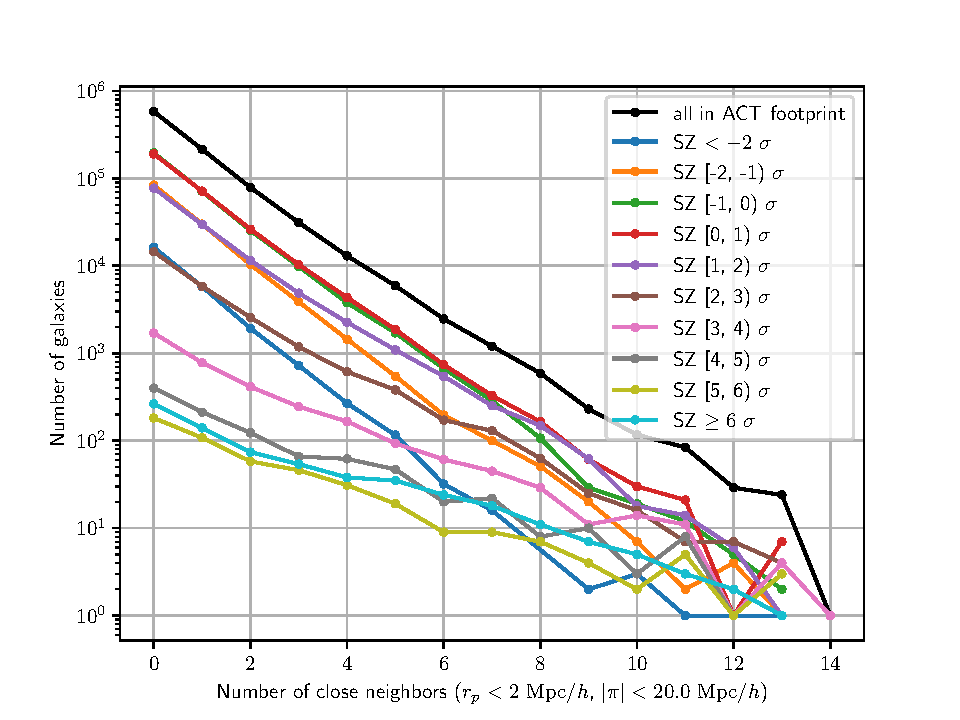
\includegraphics[width=0.495\linewidth]{fig/close_neighbor_counts_cylinders-Y1_rp2_pi20.0-numbers.pdf}
    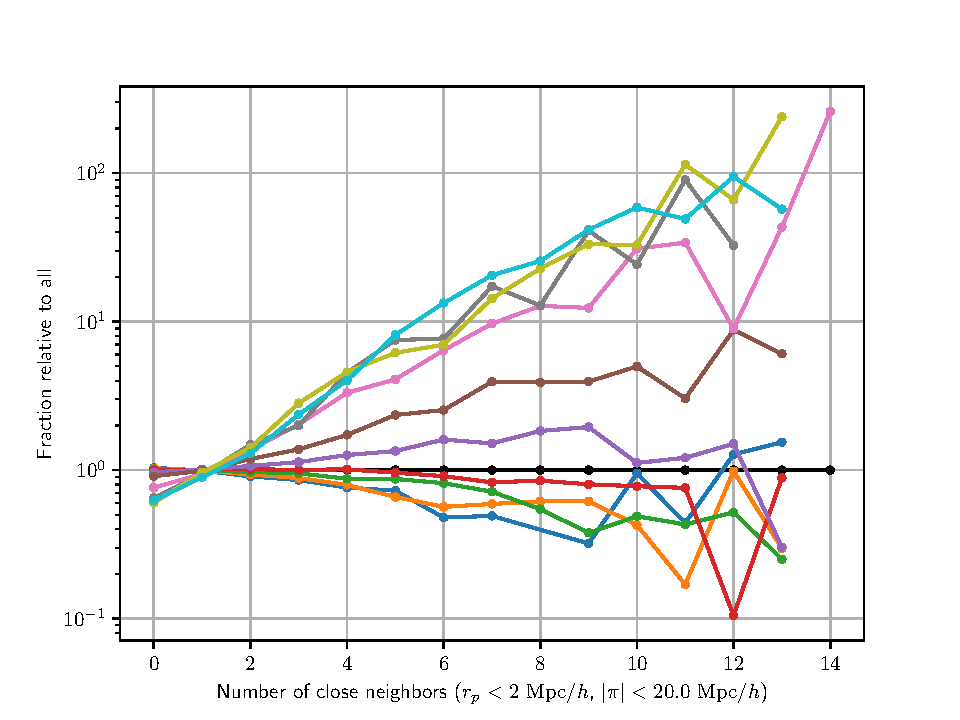
\includegraphics[width=0.495\linewidth]{fig/close_neighbor_counts_cylinders-Y1_rp2_pi20.0-rel-fraction.pdf}
    \caption[Distribution of numbers of close neighbors for LRG in different tSZ SNR bins]{Distribution of numbers of close neighbors for LRG in different tSZ SNR bins.
    Left: absolute number of galaxies in each bin with a given number of close neighbors.
    The neighbors counted are LRGs belonging to any bin.
    Right: an attempt to highlight the differences between different bins.
    ``Fraction relative to all'' is the fraction of galaxies with a given number of close neighbors in a given SNR bin, divided by the fraction of galaxies with the same number of close neighbors among the full LRG sample; see also \cref{eq:fraction-relative-to-all}.}
    \label{fig:dist-no-neighbors-cylinders-SNR-bins}
\end{figure}

We provide details on the distributions of the numbers of close neighbors in different tSZ SNR bins in \cref{fig:dist-no-neighbors-cylinders-SNR-bins}.
``Fraction relative to all'' is
\begin{equation}
    \frac{N(\text{galaxies in SNR bin with $k$ neighbors})}{N(\text{galaxies in SNR bin})} \times \frac{N(\text{all galaxies})}{N(\text{all galaxies with $k$ neighbors})} \label{eq:fraction-relative-to-all}
\end{equation}
We obtained them by
\begin{itemize}
    \item finding all the unique close galaxy pairs obeying the desired condition (\cref{sec:method-near-neighbor-search-cylinder} details the numerical method);
    \item counting occurrences of each galaxy in the resulting array of pair member indices, which gives the number of close neighbors for that galaxy;
    \item counting how many galaxies have each number of neighbors (discrete histogram, e.g. {\tt numpy.bincount}) for the full LRG sample;
    \item dividing the galaxies into SNR bins and repeating the previous step in each bin.
\end{itemize}

\section{Efficient method for near-neighbor search in cylinders}
\label{sec:method-near-neighbor-search-cylinder}

In this section, we describe our methodology for efficient search of close-neighbor galaxy pairs with different limits on parallel ($r_{\parallel,\max}$) and perpendicular ($r_{\perp,\max}$) separations within the pair.
We define $r_\parallel$ and $r_\perp$ as components of the pair separation vector $\bm{r}_2 - \bm{r}_1$ with respect to the line-of-sight direction $\hat n$.
In periodic boxes, this direction is typically fixed (flat-sky approximation).
In the more complex case of a large realistic survey accounting for the curved sky, we choose $\hat n$ along the direction to the midpoint of the pair, $\bm{r}_1 + \bm{r}_2$.

We assume flat FLRW cosmology (as is DESI fiducial cosmology for comoving distance computations and coordinate conversion), allowing us to convert to 3D Cartesian space.

We build upon the $k$-d ($k$-dimensional) tree --- an efficient data structure for searching for pairs closer than a given $k$-d Euclidean distance, or more generally with any other $p$-norm with $p\ge 1$ for $k$-dimensional vectors:
\begin{equation}
    \norm{\bm{v}}_p \equiv \qty(\sum_{i=1}^k \abs{v_i}^p)^{1/p}. \label{eq:p-norm}
\end{equation}
The $p\rightarrow +\infty$ limit (hereafter $p=\infty$ for brevity) is the maximum norm, which will be useful:
\begin{equation}
    \norm{\bm{v}}_\infty \equiv \max\qty(\abs{v_1}, \dots, \abs{v_k}). \label{eq:max-p-infty-norm}
\end{equation}
The $k$-d tree pair-finding algorithm relies on the fact that $\norm{x}_p \ge \abs{x_i}$ for any component index $i$.
Many other distance metrics do not have such property.

Of course, any pair of galaxies with $\abs{r_{\parallel}} \le r_{\parallel,\max}$ and $r_\perp \le r_{\perp,\max}$ also satisfy $\abs{\bm{r}_2 - \bm{r}_1} \le \sqrt{r_{\parallel,\max}^2 + r_{\perp,\max}^2}$.
The latter criterion can be straightforwardly used for pair searching with a $k$-d tree, but this step produces extra pairs.
We then need to store their information, compute $r_\parallel, r_\perp$ strictly for them, check the exact condition, and discard a large fraction of the pre-selected pairs (especially if the cylinder aspect ratio is very unequal, like $r_{\parallel,\max} = 10 \times r_{\perp,\max}$ in our use cases).
Next, we explain several ideas to optimize the pair pre-selection with $k$-d tree, e.g., for the sake of memory usage.

\subsection{Fixed line of sight}

With a fixed line-of-sight direction, we can align one of the coordinate axes with it by rotation if they do not match already.
Let us assume $\hat n = \hat z$ in the remainder of this subsection.
Then we can scale the parallel and perpendicular separations independently via
\begin{align}
    x' &= a_\perp x, \\
    y' &= a_\perp y, \\
    z' &= a_\parallel z.
\end{align}
In principle, we can use $a_\perp = 1/r_{\perp,\max},a_\parallel = 1/r_{\parallel,\max}$ and define a custom norm
\begin{equation}
    \norm{\bm{\Delta r'}}_{\rm custom} \equiv \max\qty[\sqrt{\qty(\Delta x')^2 + \qty(\Delta y')^2}, \abs{\Delta z'}],
\end{equation}
which exactly defines the cylinder we want and maintains the property of being not less than the absolute difference in any coordinates, so $k$-d tree could work with it.
However, the {\tt scipy} \citep{2020SciPy-NMeth, scipy_8092679} implementation only supports the $p$-norm, \cref{eq:p-norm}, including the $p=\infty$ case, \cref{eq:max-p-infty-norm}.
This gives two options of imperfect pre-selection:

\begin{enumerate}
    \item $\norm{\bm{\Delta r'}}_\infty<1$ criterion with $a_\perp = 1/r_{\perp,\max},a_\parallel = 1/r_{\parallel,\max}$.
    This is, in essence, fitting a cube over a cylinder with a height ($h$) equal to its diameter ($2R$), and the ratio of volumes is $4/\pi$.
    \item using the Euclidean ($p=2$) norm, essentially fitting a sphere over the cylinder.
    The optimal aspect ratio is less obvious than in the previous case, but the minimum sphere-to-cylinder volume ratio is $\sqrt{3}$ for $h/R=\sqrt{2}$.
    $\sqrt{3}>4/\pi$ so this variant seems worse.
\end{enumerate}

As a result, we used the first option and filtered the resulting pairs using the criterion $\qty(\Delta x)^2 + \qty(\Delta y)^2 \le r_{\perp,\max}^2$, because $\abs{\Delta z}\le r_{\parallel,\max}$ is already guaranteed.

\subsection{Varying (midpoint) line of sight}

The problem is more challenging with varying line-of-sight direction $\hat n$ because it does not allow rescaling the component separately as straightforwardly.

However, it is possible to erase information along the line of sight by projecting each galaxy onto the unit sphere:
\begin{align}
    x' &= x/r, \\
    y' &= y/r, \\
    z' &= z/r.
\end{align}

If we define $\Theta = \angle\qty(\bm r_1, \bm r_2)$, the distance between the corresponding points $\bm r'_1,\bm r'_2$ on the unit sphere is $2\sin(\Theta/2)$ whereas we prove that
\begin{equation}
    r_\perp \ge \min\qty(r_1, r_2) \sin\Theta.
\end{equation}
Thus, if we have a galaxy sample with a minimum distance to the origin $r_{\min}\ne 0$, we can use the unit sphere to apply a meaningful, albeit not a perfect pre-filter in $r_\perp$.
To avoid excluding extra pairs, the (Euclidean) distance limit on the unit sphere should be slightly larger than $\sin\Theta_{\max} = r_{\perp,\max}/r_{\min}$.
This is a 2-dimensional surface of the sphere embedded in 3-dimensional space.

Our addition is a fourth dimension for the radial coordinate:
\begin{equation}
    w' = a \times r.
\end{equation}
It can allow to apply a filter in $r_\parallel$ because
\begin{equation}
    \abs{r_\parallel} \ge \abs{r_2 - r_1},
\end{equation}
although it is imperfect too.

Like with the fixed line of sight, for the combination of the $r_\perp$ and $r_\parallel$ constraints without re-implementing the $k$-d tree, we should choose between the maximum ($p=\infty$) and Euclidean ($p=2$) norms.
Similarly, the implementation with the maximum norm has more straightforward rescaling factors.
Efficiency estimates are harder now, but the implementation with the maximum norm is more straightforward and it gave a marginally better pre-selection than with the Euclidean norm for our data, as we show in \cref{tab:close-pair-selection-methods-comparison}.
Both 4-dimensional embedding variants give a significantly stricter selection than the 3D distance filter and the $r_\perp$-only selection with the sphere embedding in 3D.

\begin{table}
    \centering
    \begin{tabular}{|c|c|c|}
        \hline
        Number of pairs & $r_\perp<2, \abs{r_\parallel}<20$ & $r_\perp<3, \abs{r_\parallel}<30$ \\
        \hline
        Simple distance & $1.15\E{7}$ & $3.05\E{7}$ \\
        Sphere embedded in 3D & $6.27\E{6}$ & $1.37\E{7}$ \\
        4D embedding, $p=2$ & $1.16\E{6}$ & $2.70\E{6}$ \\
        4D embedding, $p=\infty$ & $1.11\E{6}$ & $2.51\E{6}$ \\
        \hline
        Complete condition & $4.40\E{5}$ & $9.25\E{5}$ \\
        \hline
    \end{tabular}
    \caption[Comparison of different pair pre-selection methods' efficiency]{Resulting number of pairs for different close-pair pre-selection methods for our two criteria for DESI DR1 LRG (curved sky) with redshifts $0.4<z<0.85$.
    The distances are in $\ihMpc$.}
    \label{tab:close-pair-selection-methods-comparison}
\end{table}